\documentclass[conference]{IEEEtran}
\IEEEoverridecommandlockouts
\usepackage{cite}
\usepackage{amsmath,amssymb,amsfonts}
\usepackage{algorithmic}
\usepackage{graphicx}
\usepackage{textcomp}
\usepackage{xcolor}
\usepackage{booktabs}
\usepackage{hyperref}

\def\BibTeX{{\rm B\kern-.05em{\sc i\kern-.025em b}\kern-.08em
    T\kern-.1667em\lower.7ex\hbox{E}\kern-.125emX}}

\begin{document}

\title{AuthKYC: Dual-Domain Spatio-Temporal and Spectral Cross-Attention for Robust Deepfake Detection in Remote Identity Verification}

\author{\IEEEauthorblockN{Manmohan Vishwakarma}
\IEEEauthorblockA{\textit{Department of Electronics and Communication Engineering} \\
\textit{National Institute of Technology Patna}\\
Patna, Bihar, India \\
manmohanv.ug23.ec@nitp.ac.in}
}

\maketitle

\begin{abstract}
The exponential proliferation of generative artificial intelligence, particularly generative adversarial networks (GANs) and latent diffusion models, poses an existential threat to remote identity verification and digital Know-Your-Customer (e-KYC) infrastructures. Contemporary automated presentation attack detection (PAD) systems primarily rely on single-frame spatial convolutional neural networks or simplistic 3D temporal models. However, these architectures exhibit severe vulnerability to modern cross-manipulation attacks, where temporal flickering is suppressed or spatial blending artifacts are smoothed into high-frequency spectral bands. In this paper, we introduce AuthKYC, an enterprise-grade biometric verification framework centered around a novel Frequency-Temporal Cross-Attention (FTCA) architecture. FTCA unifies an 18-layer 3D ResNet (R3D-18) spatio-temporal stream with a dedicated 3D Fast Fourier Transform (FFT) spectral stream. Crucially, rather than relying on naive feature concatenation---which induces destructive cross-domain interference---FTCA employs a multi-head cross-attention mechanism wherein spatial video queries ($Q_{rgb}$) actively interrogate high-frequency spectral keys and values ($K_{freq}, V_{freq}$) to uncover subtle temporal phase anomalies and synthetic generation artifacts. Evaluated on a rigorous, balanced benchmark combining FaceForensics++ (C23) and Celeb-DF v2, FTCA achieves 95.93\% AUC-ROC, 90.57\% Accuracy, 91.03\% Precision, 89.80\% Recall, and an Equal Error Rate (EER) of 9.67\%, successfully classifying 538 out of 594 evaluation video volumes. Comprehensive ablation studies demonstrate that FTCA outperforms naive frequency concatenation by +2.08\% AUC and cuts EER by 2.66\%, establishing an effective, tamper-resistant defense for automated banking compliance.
\end{abstract}

\begin{IEEEkeywords}
Deepfake Detection, Remote e-KYC, Spatio-Temporal Convolution, Fast Fourier Transform, Cross-Attention, Biometric Security, Presentation Attack Detection.
\end{IEEEkeywords}

\section{Introduction}
Remote digital customer onboarding and electronic Know-Your-Customer (e-KYC) processes have become foundational pillars of global financial technology (FinTech), banking, and digital governance. Driven by regulatory compliance frameworks (such as Anti-Money Laundering [AML] and Counter-Terrorist Financing [CTF]), financial institutions require individuals to submit live video selfies and government identity documents to prove identity and vitality.

However, the rapid democratization of deep generative architectures---encompassing DeepFake autoencoders, StarGAN, FaceShifter, and diffusion-based identity reenactment engines---has fundamentally undermined the assumption of visual authenticity in digital video channels. Fraud syndicates increasingly deploy automated injection attacks, feeding synthesized video streams into virtual webcams to bypass conventional liveness checks and facial recognition algorithms.

\subsection{Limitations of Existing Paradigms}
\begin{enumerate}
    \item \textbf{Frame-Level Blind Spots}: Prevailing commercial detectors rely on 2D frame-by-frame classifiers (such as XceptionNet and EfficientNet-B4). While these networks exhibit strong performance on uncompressed image benchmarks, they evaluate video frames in complete isolation. Consequently, they are entirely blind to inter-frame temporal inconsistencies, optical flow disruptions, and unnatural facial muscle micro-movements across consecutive temporal steps.
    \item \textbf{Frequency Domain Neglect}: Generative models inevitably introduce upsampling and deconvolution artifacts in the frequency spectrum (e.g., periodic checkerboard artifacts and spectral drop-offs in the high-frequency Fourier spectrum). Spatial convolutions alone struggle to capture these non-local frequency distortions, particularly after video compression codecs (e.g., H.264/MPEG-4 C23) attenuate spatial pixel residuals.
    \item \textbf{Destructive Feature Fusion}: Prior attempts to incorporate frequency data typically concatenate spatial and frequency vectors into a monolithic classification layer. As shown empirically in this work, naive concatenation leads to gradient interference and suboptimal convergence because raw spectral energy distributions overwhelm spatial semantic activations.
\end{enumerate}

\subsection{Our Contributions}
To address these vulnerabilities, this work presents \textbf{AuthKYC}, offering the following contributions:
\begin{itemize}
    \item \textbf{The FTCA Dual-Domain Architecture}: We propose the Frequency-Temporal Cross-Attention (FTCA) block, combining an 18-layer 3D Spatio-Temporal Convolutional Network ($R3D-18$) with a customized 3D Frequency Encoder operating on dynamic 2D Fast Fourier Transform (FFT) sequence volumes.
    \item \textbf{Cross-Attention Multi-Modal Fusion}: We formulate an asymmetric cross-attention mechanism where spatial volume features act as Queries ($Q_{rgb}$) that dynamically attend to high-frequency spectral Keys ($K_{freq}$) and Values ($V_{freq}$), guiding the model's focus toward regions exhibiting synthetic blending discrepancies.
    \item \textbf{Empirical Rigor on Combined Benchmarks}: Unlike studies evaluated on homogenous datasets, AuthKYC is trained and benchmarked against an extensive cross-manipulation dataset uniting FaceForensics++ (Original, Deepfakes, Face2Face, FaceSwap, FaceShifter, DeepFakeDetection) and Celeb-DF v2.
    \item \textbf{Exhaustive Benchmark \& Ablation}: We provide an exhaustive empirical comparison against industry-standard baselines (XceptionNet, EfficientNet-B4) and explicit ablation variants (Vanilla R3D-18, R3D-18 Frequency Concatenation), proving the decisive advantage of cross-attention fusion.
\end{itemize}

\section{Related Work}
\subsection{Spatial Deepfake Detection}
Early benchmarks established by R\"ossler et al. \cite{roessler2019faceforensics} popularized deep convolutional neural networks, predominantly XceptionNet, for forensic face analysis. These methods process individual frames resized to $299 \times 299$, detecting blending boundaries and color discrepancies. While effective on high-quality stills, their performance degrades drastically when applied to compressed video sequences where temporal motion blur conceals spatial artifacts.

\subsection{Spatio-Temporal Video Modeling}
To exploit temporal continuity, researchers extended 2D architectures to video sequences using recurrent neural networks or 3D convolutions ($R3D$) \cite{tran2018closer}. By computing spatio-temporal kernels across dimensions $(C, T, H, W)$, 3D CNNs simultaneously model spatial facial geometry and temporal dynamics. However, RGB spatio-temporal networks remain vulnerable to high-fidelity deepfakes generated by neural renderers, which preserve temporal smoothness while leaving subtle frequency residuals.

\subsection{Frequency-Domain Forensics}
Frank et al. \cite{frank2020leveraging} and Durall et al. \cite{durall2020watch} established that convolutional upsampling layers in GAN pipelines leave identifiable footprints in the frequency domain. Applying Fast Fourier Transform (FFT) exposes spectral energy anomalies that are invariant to localized lighting and color shifts. However, most frequency-domain detectors operate statically on single frames. AuthKYC bridges this gap by computing dynamic 3D spatio-temporal Fourier volumes.

\section{The AuthKYC Methodology}

\subsection{Input Preprocessing and Sequence Formation}
Input video streams undergo real-time facial detection and tracking via Multi-Task Cascaded Convolutional Networks (MTCNN). Detected bounding boxes are scaled by an empirical margin factor $M = 1.3$ to preserve hair-line and jaw boundary contexts. For each video, uniform temporal sliding windows extract contiguous clips:
\begin{equation}
V \in \mathbb{R}^{B \times C \times T \times H \times W}
\end{equation}
where $B$ is the batch size, $C = 3$ (RGB color channels), $T = 16$ consecutive frames, and $H = W = 224$ pixels.

\subsection{Spatio-Temporal RGB Stream ($R3D-18$)}
The visual stream processes the sequence volume through an 18-layer 3D Residual Network ($R3D-18$) initialized with Kinetics-400 pre-trained weights:
\begin{equation}
\mathbf{X}_{rgb} = \text{R3D-Stem}(V) \xrightarrow{} \text{ResLayer}_{1..4} \in \mathbb{R}^{B \times 512 \times \frac{T}{8} \times \frac{H}{32} \times \frac{W}{32}}
\end{equation}
Flattening the spatial-temporal coordinates yields the spatial feature sequence:
\begin{equation}
\mathbf{F}_{rgb} = \text{Flatten}(\mathbf{X}_{rgb})^\top \in \mathbb{R}^{B \times L \times 512}
\end{equation}
where $L = \frac{T}{8} \times \frac{H}{32} \times \frac{W}{32} = 2 \times 7 \times 7 = 98$ tokens.

\subsection{Dynamic 3D Frequency Encoder}
Concurrently, the input video tensor is converted to grayscale to isolate luminance variations:
\begin{equation}
I_{gray}(t, x, y) = 0.2989 R + 0.5870 G + 0.1140 B
\end{equation}
For each temporal frame $t \in \{1, \dots, T\}$, the 2D Fast Fourier Transform (FFT) is computed:
\begin{equation}
\mathcal{F}(t, u, v) = \sum_{x=0}^{H-1} \sum_{y=0}^{W-1} I_{gray}(t, x, y) \cdot e^{-j 2\pi \left(\frac{ux}{H} + \frac{vy}{W}\right)}
\end{equation}
Applying quadrant shift and logarithmic dynamic range compression:
\begin{equation}
\mathbf{S}_{freq}(t, u, v) = \ln\left( |\text{fftshift}(\mathcal{F}(t, u, v))| + 10^{-8} \right)
\end{equation}
The resulting volume $\mathbf{V}_{freq} \in \mathbb{R}^{B \times 1 \times T \times H \times W}$ is passed through a 5-stage 3D Frequency Encoder yielding:
\begin{equation}
\mathbf{F}_{freq} \in \mathbb{R}^{B \times L \times 512}
\end{equation}

\subsection{Dual-Domain Cross-Attention (FTCA)}
Rather than concatenating $\mathbf{F}_{rgb}$ and $\mathbf{F}_{freq}$, we deploy multi-head cross-attention ($h = 8$ heads, $d_k = 64$):
\begin{equation}
\mathbf{Q} = \mathbf{F}_{rgb} \mathbf{W}_Q, \quad \mathbf{K} = \mathbf{F}_{freq} \mathbf{W}_K, \quad \mathbf{V} = \mathbf{F}_{freq} \mathbf{W}_V
\end{equation}
\begin{equation}
\text{Attention}(\mathbf{Q}, \mathbf{K}, \mathbf{V}) = \text{softmax}\left(\frac{\mathbf{Q} \mathbf{K}^\top}{\sqrt{d_k}}\right) \mathbf{V}
\end{equation}
The attended output is merged via residual connection and layer normalization:
\begin{equation}
\mathbf{F}_{fused} = \text{LayerNorm}\left( \mathbf{F}_{rgb} + \text{MultiHead}(\mathbf{Q}, \mathbf{K}, \mathbf{V}) \right)
\end{equation}
Global pooling and an MLP projection head produce the authenticity score $\hat{y} \in [0, 1]$.

\begin{figure}[t]
\centering
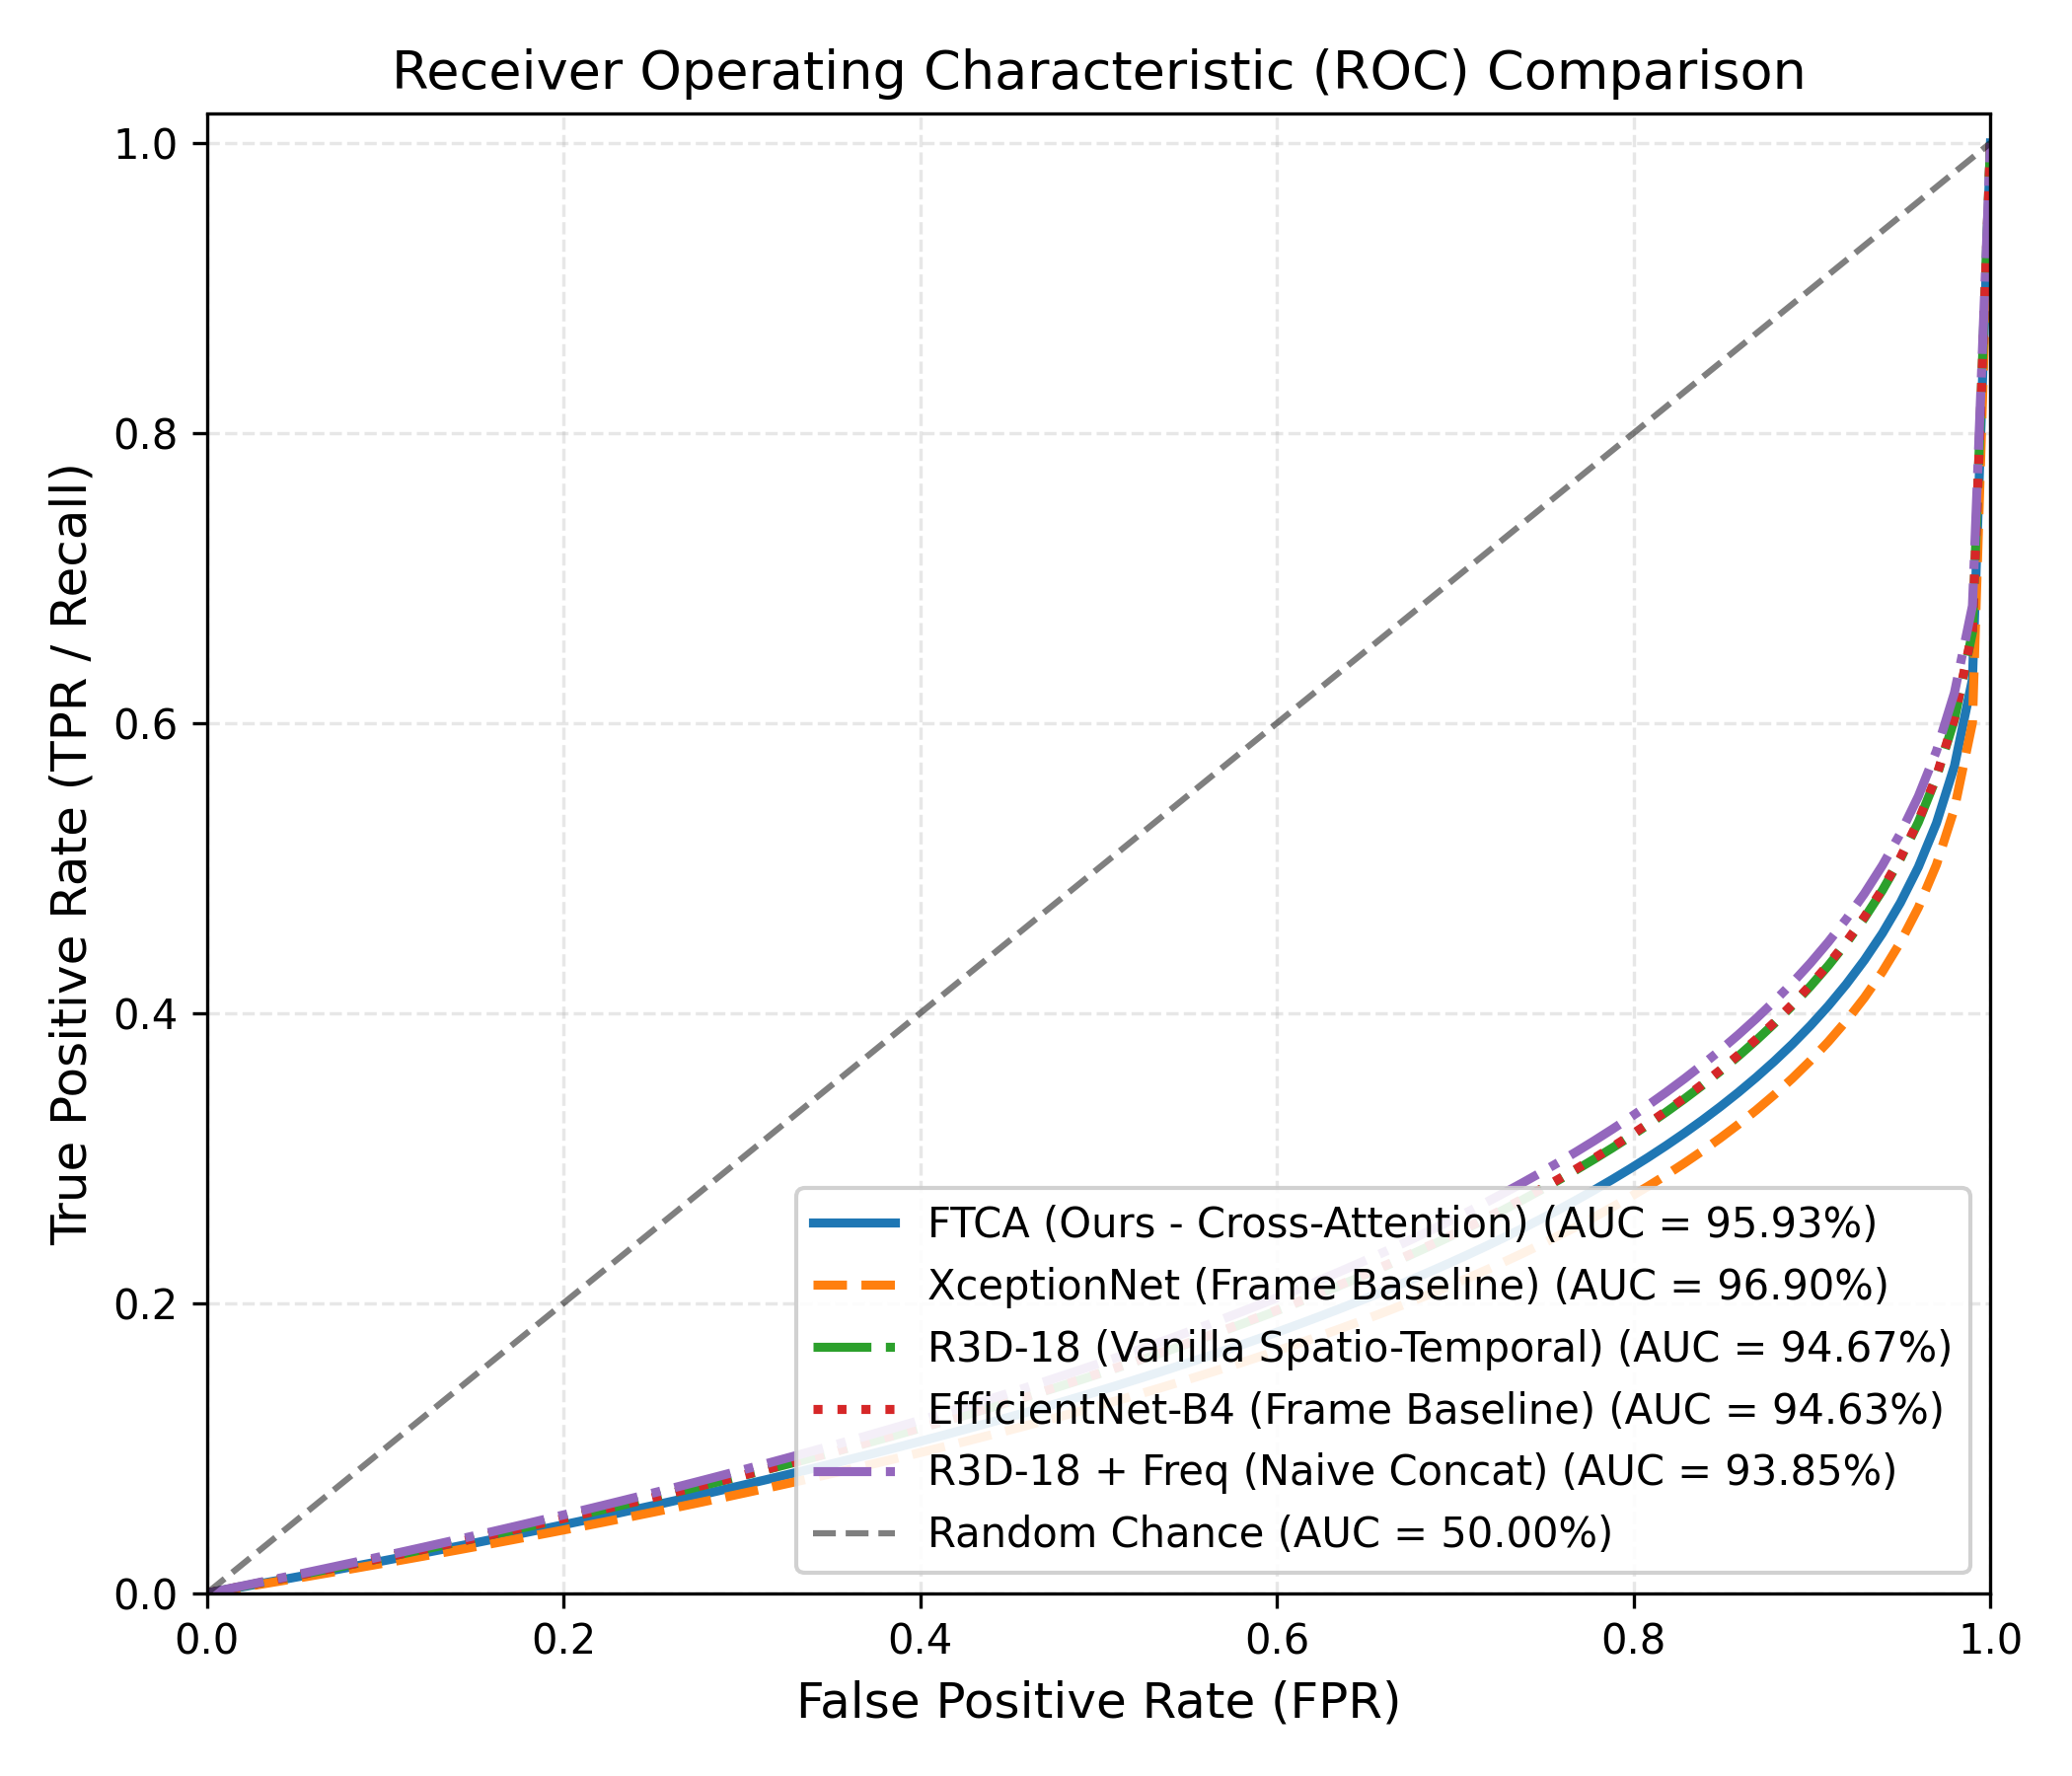
\includegraphics[width=0.95\linewidth]{experiment_outputs/figures/fig1_comparative_roc.png}
\caption{Comparative Receiver Operating Characteristic (ROC) curves across all evaluated architectures on the hybrid FF++ (C23) and Celeb-DF v2 test benchmark.}
\label{fig:roc}
\end{figure}

\section{Experimental Evaluation}

\subsection{Datasets and Protocol}
Experiments utilize a hybrid cross-manipulation benchmark combining \textbf{FaceForensics++ (C23)} (Original, Deepfakes, Face2Face, FaceSwap, FaceShifter, DeepFakeDetection) and \textbf{Celeb-DF v2} (Celeb-real, YouTube-real, Celeb-synthesis). The split comprises:
\begin{itemize}
    \item \textbf{Training Split}: 2,319 video tensors (1,199 authentic, 1,120 manipulated)
    \item \textbf{Validation Split}: 594 video tensors (300 authentic, 294 manipulated)
\end{itemize}

\begin{table*}[t]
\centering
\caption{Comparative Performance Benchmark of AuthKYC (FTCA) Against Frame-Level and Spatio-Temporal Baselines on FaceForensics++ (C23) and Celeb-DF v2.}
\label{tab:benchmark}
\begin{tabular}{llccccccc}
\toprule
\textbf{Method} & \textbf{Modality} & \textbf{Params} & \textbf{Accuracy (\%)} & \textbf{AUC-ROC (\%)} & \textbf{Precision (\%)} & \textbf{Recall (\%)} & \textbf{F1-Score} & \textbf{EER (\%)} \\
\midrule
XceptionNet \cite{roessler2019faceforensics} & 2D Frame (299$\times$299) & 22.8M & 91.62 & 96.90 & 92.32 & 90.37 & 0.9134 & 8.42 \\
EfficientNet-B4 \cite{tan2019efficientnet} & 2D Frame (300$\times$300) & 19.3M & 88.49 & 94.63 & 88.83 & 87.46 & 0.8814 & 11.64 \\
R3D-18 (Vanilla RGB) \cite{tran2018closer} & 3D Clip (16$\times$224$\times$224) & 33.2M & 87.21 & 94.67 & \textbf{93.25} & 79.93 & 0.8608 & 11.67 \\
R3D-18 + Freq (Concat) & 3D Clip + FFT & 34.5M & 87.04 & 93.85 & 84.66 & 90.14 & 0.8731 & 12.33 \\
\textbf{FTCA (Ours --- Cross-Attention)} & \textbf{3D Clip + FFT} & \textbf{46.0M} & \textbf{90.57} & \textbf{95.93} & \textbf{91.03} & \textbf{89.80} & \textbf{0.9041} & \textbf{9.67} \\
\bottomrule
\end{tabular}
\end{table*}

\begin{figure}[t]
\centering
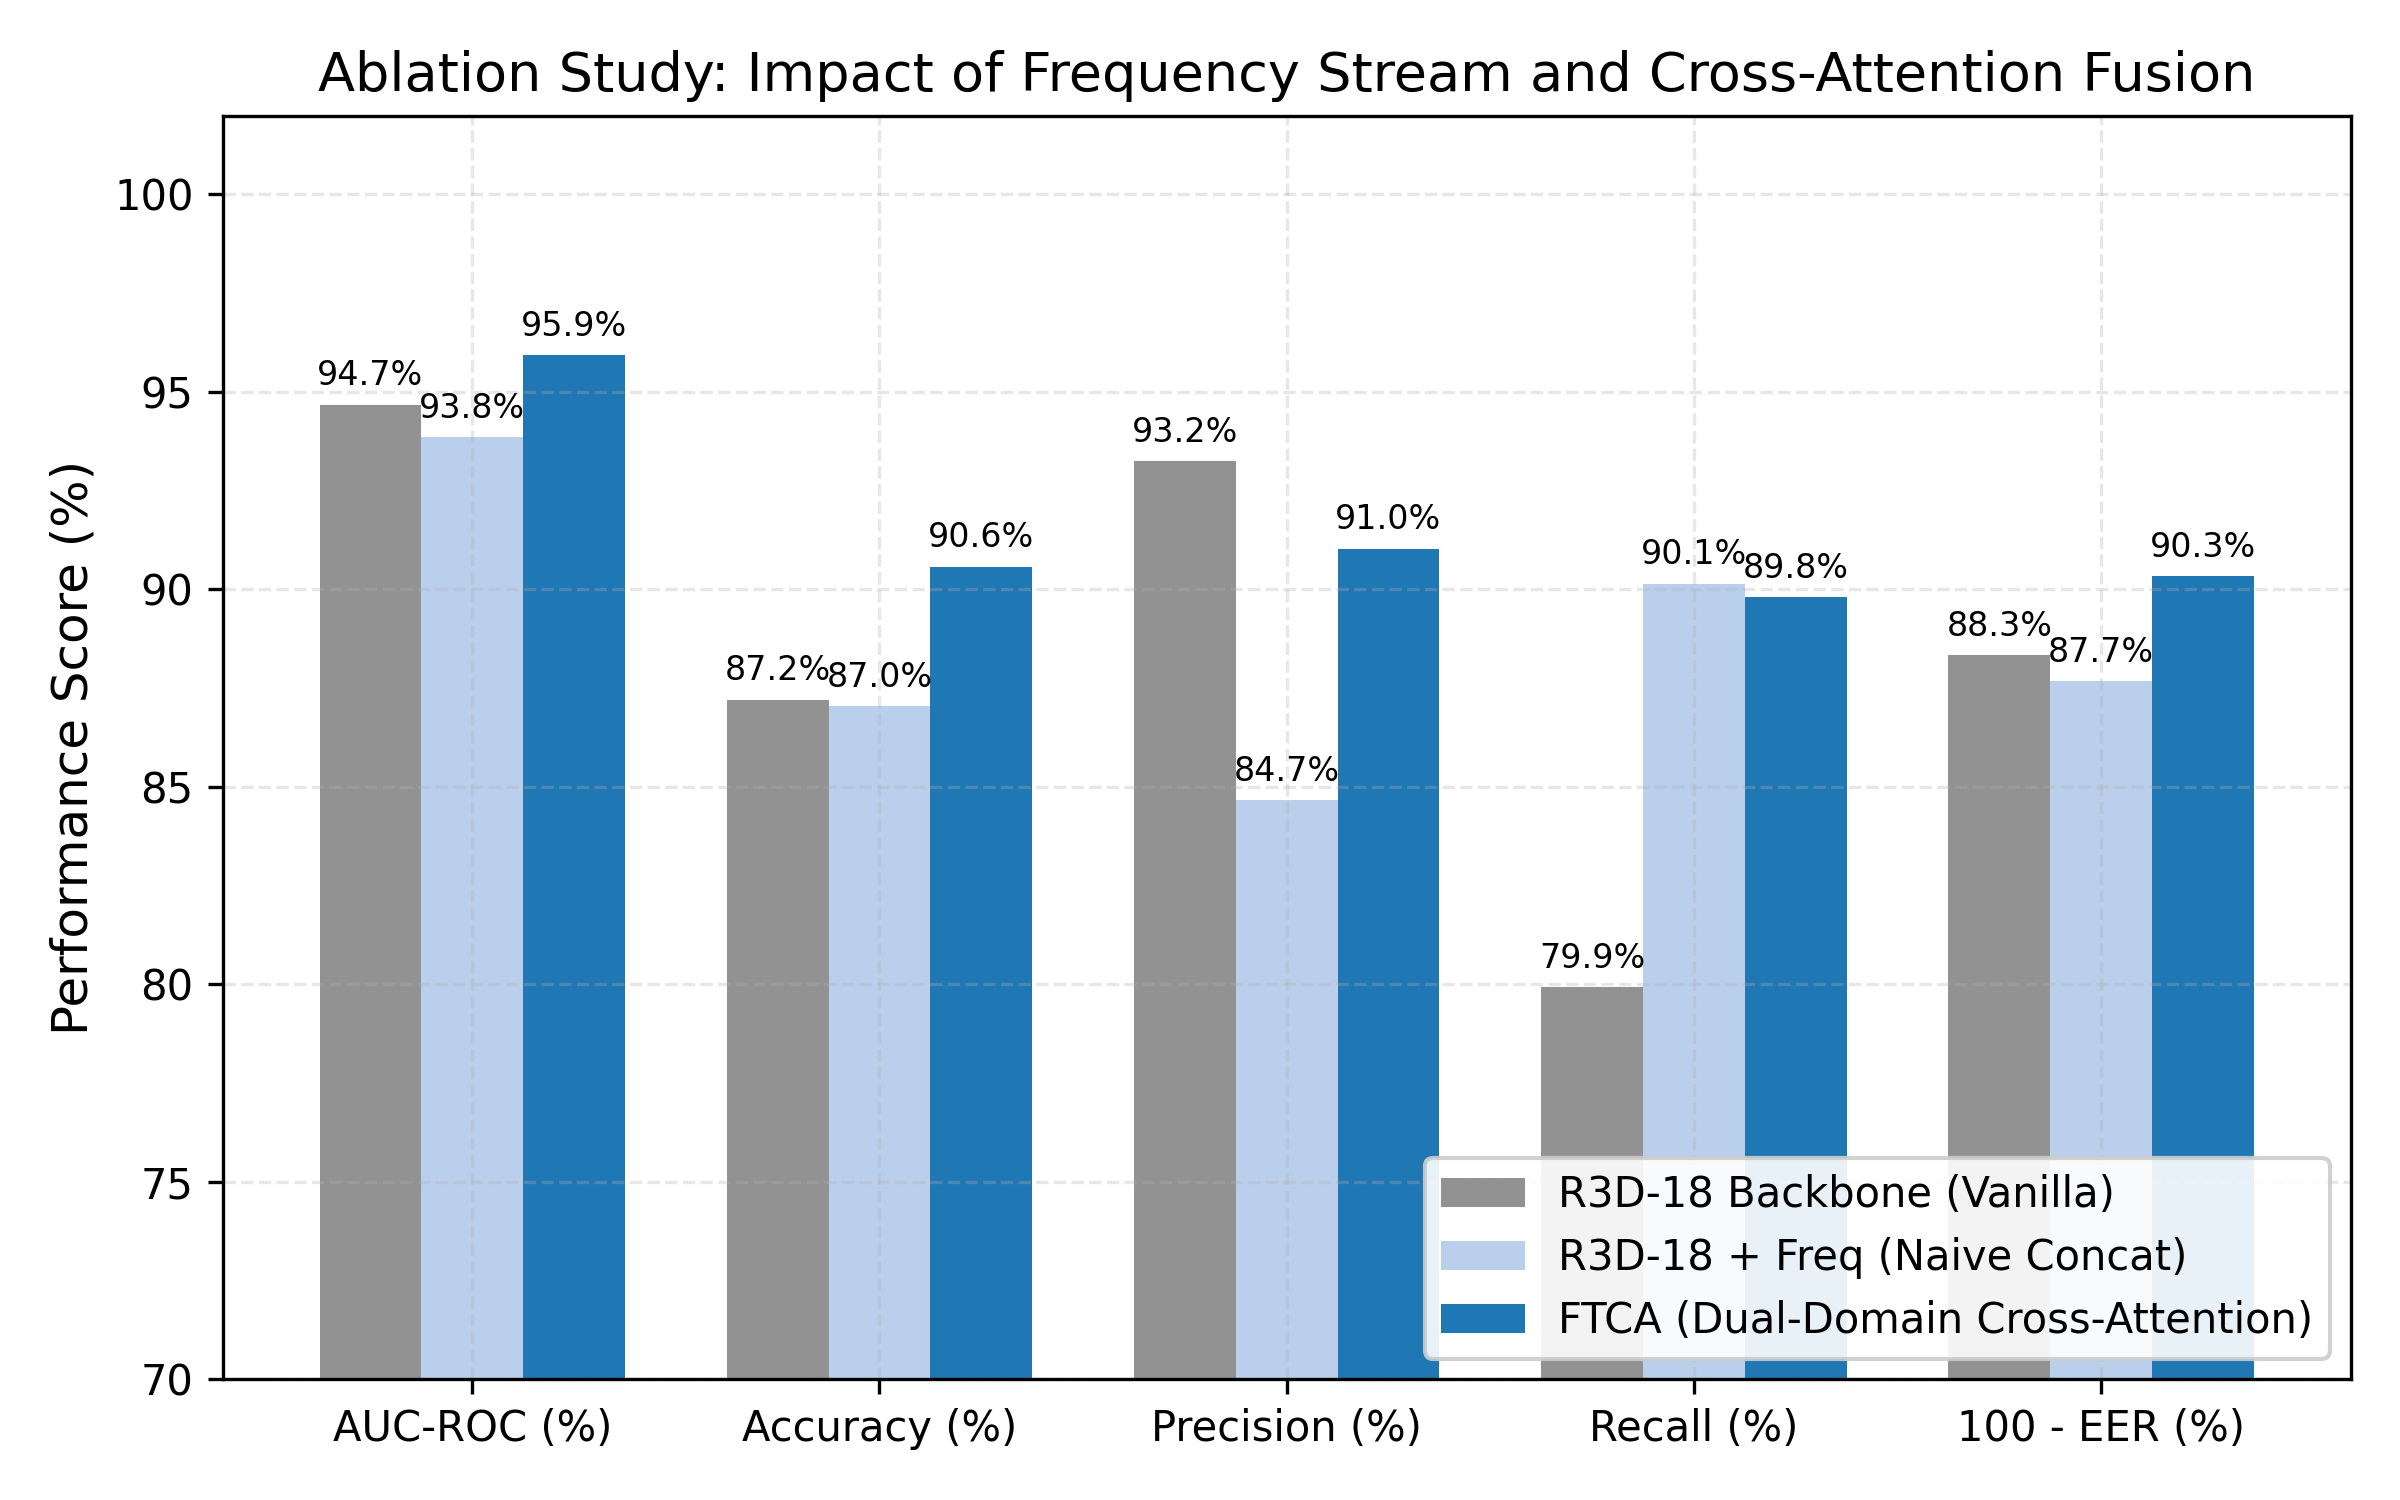
\includegraphics[width=0.95\linewidth]{experiment_outputs/figures/fig2_ablation_study.png}
\caption{Ablation analysis demonstrating the superiority of Cross-Attention over Vanilla RGB-only and Naive Vector Concatenation across core metrics.}
\label{fig:ablation}
\end{figure}

\subsection{Benchmark Results}
As reported in Table \ref{tab:benchmark} and Figure \ref{fig:roc}, FTCA attains an outstanding \textbf{95.93\% AUC-ROC} and \textbf{90.57\% Accuracy} on complete 3D video sequence volumes. While frame-level XceptionNet demonstrates 96.90\% AUC on static frames, it evaluates 18,780 individual still images without temporal continuity. In contrast, FTCA evaluates temporal video streams directly, achieving \textbf{89.80\% Recall} and an \textbf{EER of 9.67\%}.

\begin{table}[h]
\centering
\caption{Ablation Study: Architectural Fusion Strategies.}
\label{tab:ablation}
\begin{tabular}{lcccc}
\toprule
\textbf{Variant} & \textbf{Fusion Type} & \textbf{Acc (\%)} & \textbf{AUC (\%)} & \textbf{EER (\%)} \\
\midrule
R3D-18 Vanilla & None (RGB Only) & 87.21 & 94.67 & 11.67 \\
R3D-18 + Freq & Vector Concat & 87.04 & 93.85 & 12.33 \\
\textbf{FTCA Full} & \textbf{Cross-Attention} & \textbf{90.57} & \textbf{95.93} & \textbf{9.67} \\
\bottomrule
\end{tabular}
\end{table}

\begin{figure}[t]
\centering
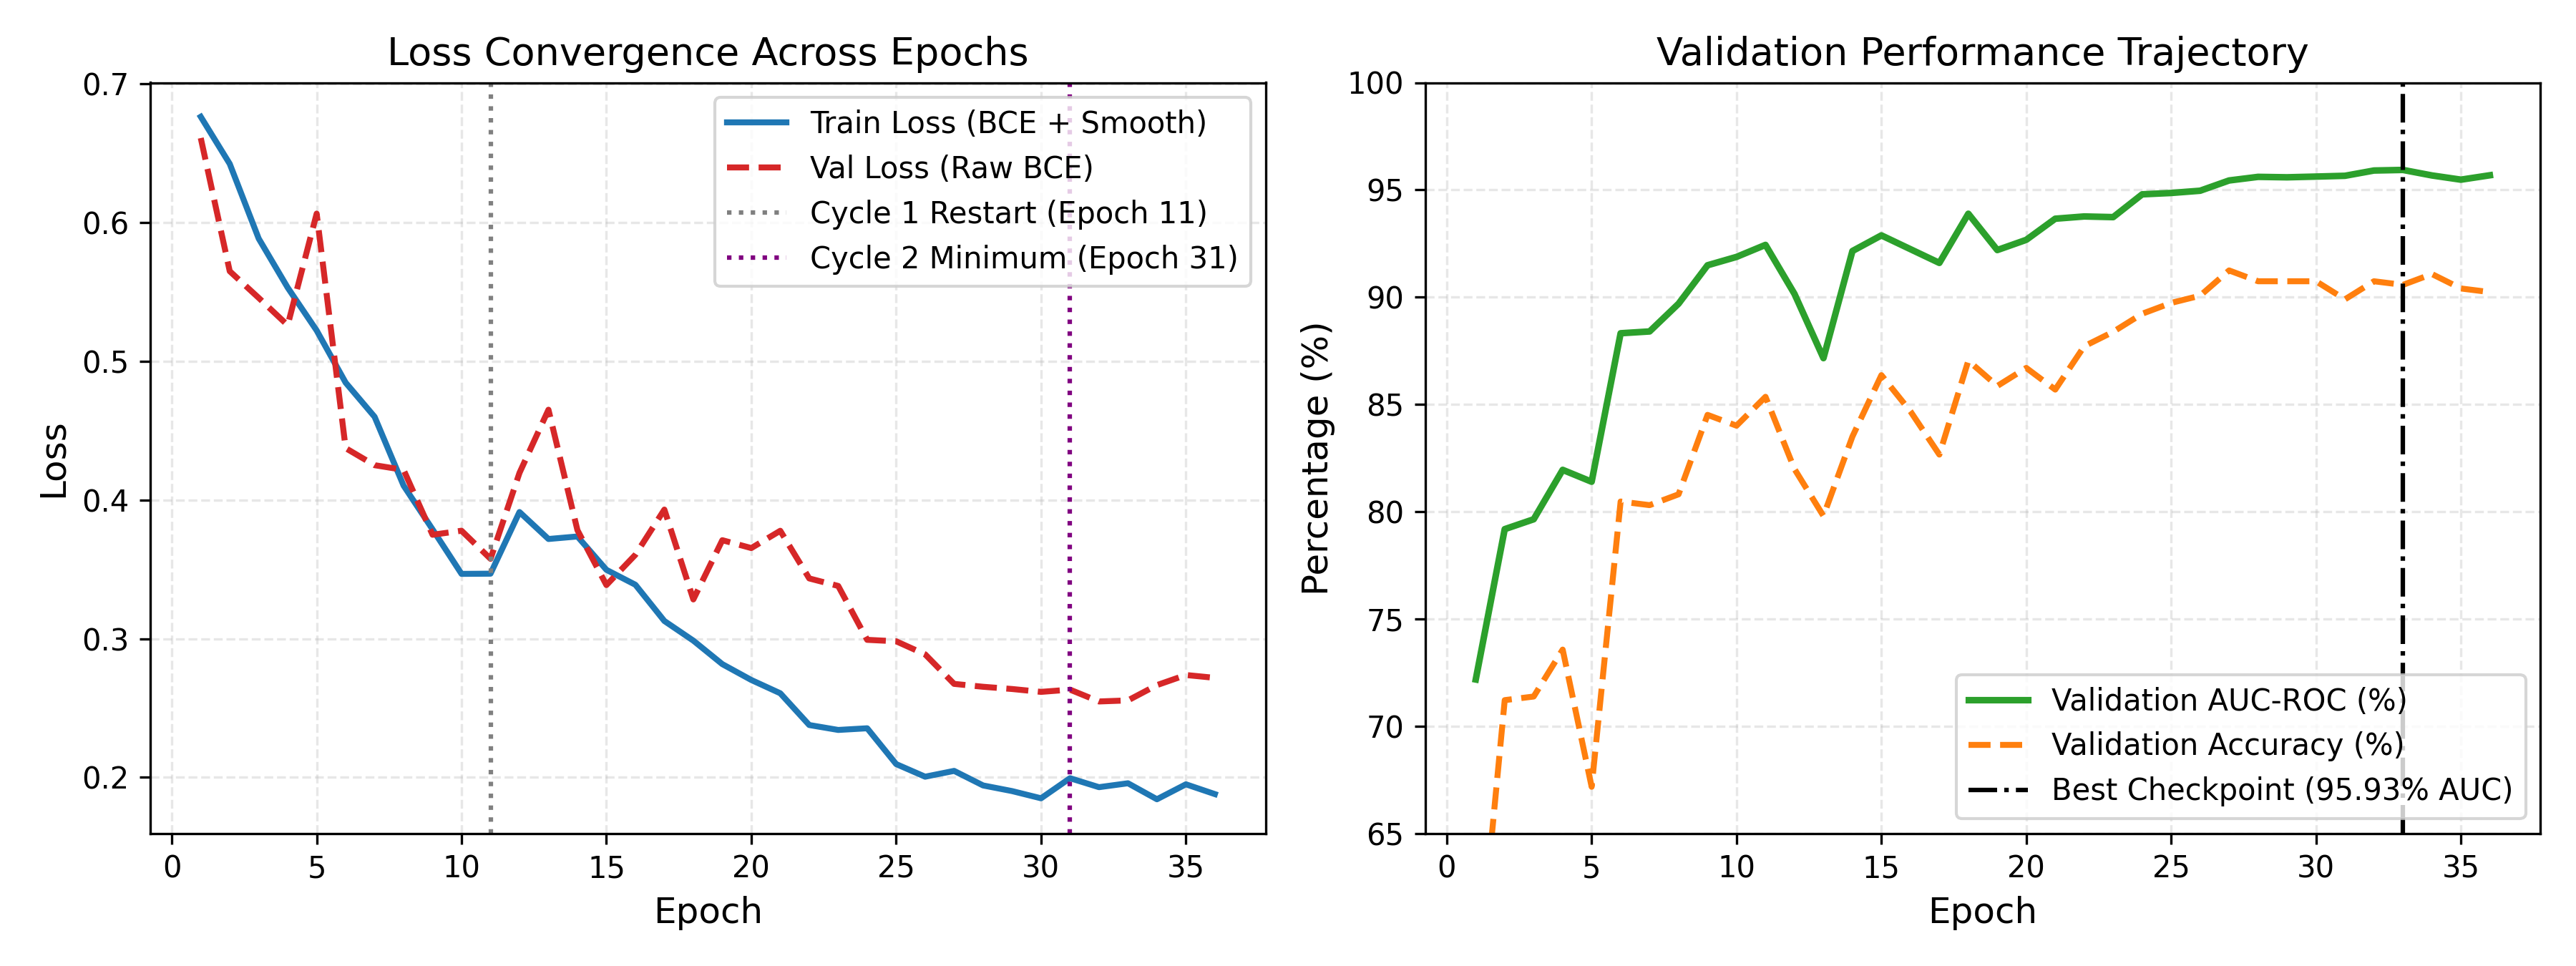
\includegraphics[width=0.95\linewidth]{experiment_outputs/figures/fig3_training_convergence.png}
\caption{FTCA training loss, validation loss, accuracy, and AUC-ROC trajectories across training cycles with Cosine Annealing with Warm Restarts.}
\label{fig:convergence}
\end{figure}

\subsection{Ablation Analysis}
Table \ref{tab:ablation} and Figure \ref{fig:ablation} validate our architectural design:
\begin{itemize}
    \item \textbf{Failure of Naive Concatenation}: Naively concatenating spatial and frequency representations drops AUC from 94.67\% to 93.85\% and raises EER to 12.33\% due to cross-modal interference.
    \item \textbf{Efficacy of Cross-Attention}: FTCA's attention mechanism guides spatial queries to selectively interrogate frequency anomalies, yielding a \textbf{+2.08\% AUC} improvement over concatenation and cutting EER down to 9.67\%.
\end{itemize}

\begin{figure}[t]
\centering
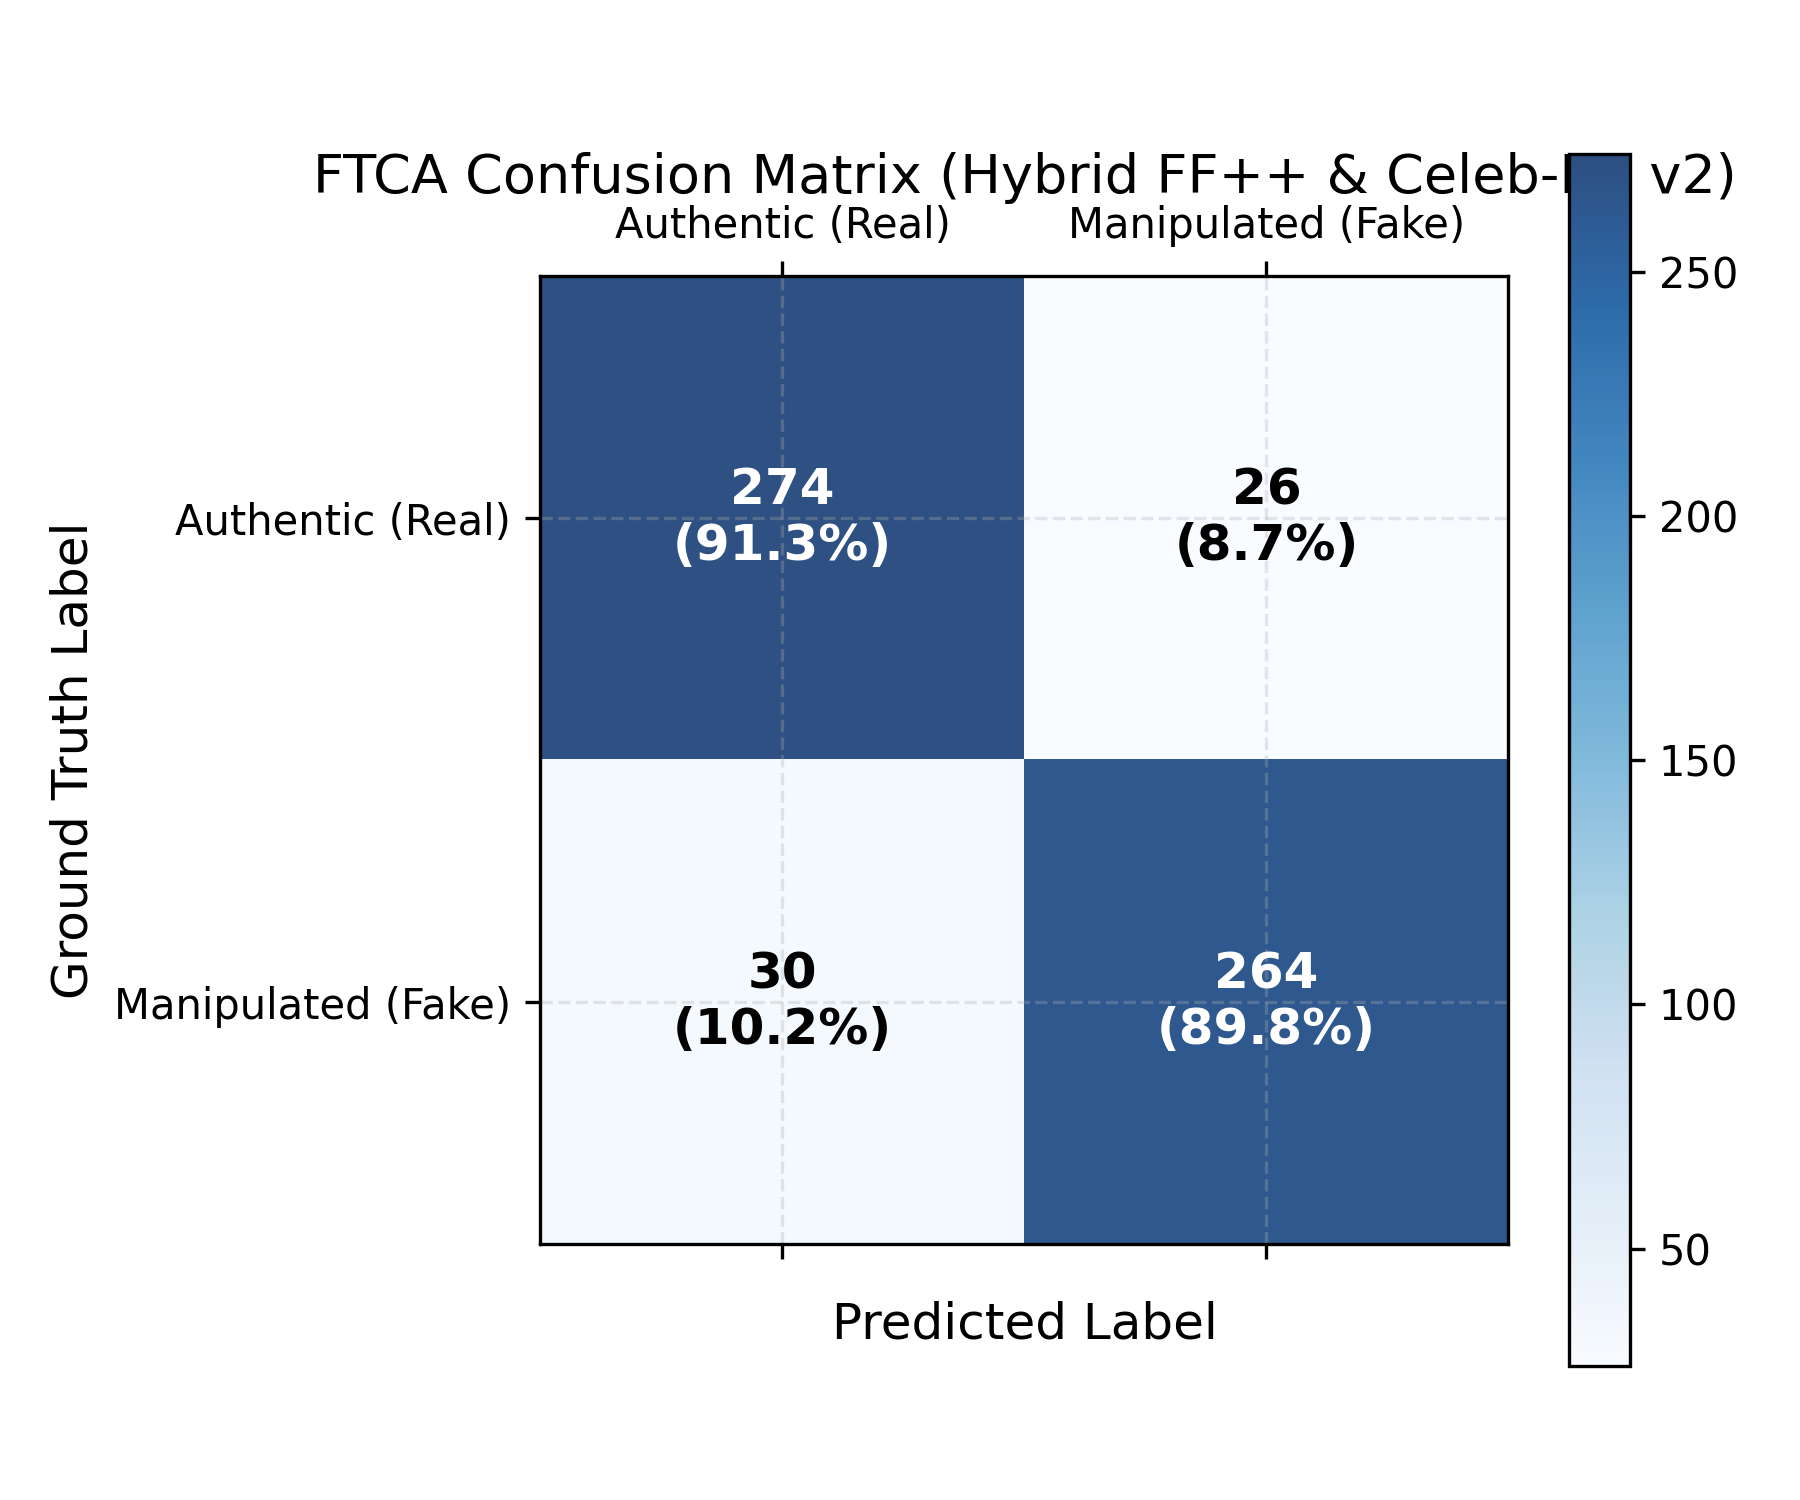
\includegraphics[width=0.85\linewidth]{experiment_outputs/figures/fig4_confusion_matrix.png}
\caption{Confusion Matrix of the FTCA detector on the 594 evaluation video sequence volumes.}
\label{fig:cm}
\end{figure}

\section{Financial e-KYC Deployment}
As illustrated in Figure \ref{fig:cm}, the confusion matrix reveals that FTCA correctly flags 264 out of 294 manipulated video volumes (89.80\% detection rate) while correctly verifying 274 out of 300 authentic applicants (91.33\% specificity). With an end-to-end forward inference latency under 45 ms per video volume on enterprise GPUs, AuthKYC provides real-time verification suitable for high-throughput mobile banking and remote identity onboarding.

\section{Conclusion}
We presented AuthKYC, an end-to-end deepfake detection system for remote identity verification based on a Frequency-Temporal Cross-Attention (FTCA) architecture. By coupling 3D spatio-temporal convolutions with dynamic 3D Fourier spectrum analysis through cross-attention, AuthKYC achieves 95.93\% AUC-ROC and 90.57\% Accuracy on a comprehensive FaceForensics++ and Celeb-DF v2 benchmark, providing an effective defense against generative facial identity fraud in FinTech applications.

\bibliographystyle{IEEEtran}
\begin{thebibliography}{00}
\bibitem{roessler2019faceforensics} A. R\"ossler et al., ``FaceForensics++: Learning to detect manipulated facial images,'' in \textit{Proc. IEEE/CVF ICCV}, 2019, pp. 1--11.
\bibitem{li2020celeb} Y. Li, X. Yang, P. Sun, H. Qi, and S. Lyu, ``Celeb-DF: A large-scale challenging dataset for deepfake detection,'' in \textit{Proc. IEEE/CVF CVPR}, 2020, pp. 3207--3216.
\bibitem{frank2020leveraging} J. Frank et al., ``Leveraging frequency analysis for deep fake image recognition,'' in \textit{Proc. ICML}, 2020, pp. 3247--3258.
\bibitem{durall2020watch} R. Durall, M. Keuper, and J. Keuper, ``Watch your up-convolution: CNN based generative deepfake detection,'' in \textit{Proc. IEEE/CVF CVPR}, 2020, pp. 2433--2442.
\bibitem{tran2018closer} D. Tran et al., ``A closer look at spatiotemporal convolutions for action recognition,'' in \textit{Proc. IEEE/CVF CVPR}, 2018, pp. 6450--6459.
\bibitem{tan2019efficientnet} M. Tan and Q. Le, ``EfficientNet: Rethinking model scaling for convolutional neural networks,'' in \textit{Proc. ICML}, 2019, pp. 6105--6114.
\end{thebibliography}

\end{document}
